
An important class of problems deal with the steady-state, i.e., where the
system after a transient time no longer evolves. The steady-state we formally
define as  
\begin{equation}
  \frac{\partial c}{\partial t}=0 
\end{equation}
implying that $c=c(x)$. In this case and for constant diffusion coefficient,
the RD-equation reduces to an ordinary differential equation
\begin{equation}
  D\frac{\d^2c}{\d x^2} + r(c)=0  
\end{equation}
This equation together with some appropriate BCs 
define a boundary value problem and is what we will study in the next few
sections. In the last optional section we explore \emph{chemotaxis} which is a phenomenon where 
cells migrate due to a signaling compound. While this is not a 
reaction-diffusion phenomenon, we can easily apply what we 
learn in the first sections and thus further extent the applications.

The boundary value problems we encounter here when $r$ is a linear function 
are examples of the \emph{Sturm-Liouville} problem. The theoretical 
framework of this general problem is very elegant and quite useful, however, we shall 
not embark on an indepth treatment here, but simply make a few references. 


\section{Linear reaction functions \label{stst:sectBVP}}
In Example \ref{ex:simplegrowth} we 
introduced an RD-equation with a simple linear reaction function, $r=kc$.  
Let us explore this example in the case where $k>0$, that is, the population
self-multiply,  
\begin{equation}
  \label{eq:simplegrowthss}
	D\frac{\d^2c}{\d x^2} + kc=0 \, \ \ \ (k>0).
\end{equation}
Since we have no time in the problem we do not have an IC, and in this first
example we apply simple Dirichlet BCs
\begin{equation}
  c(0)=c(L)=0 \, .
\end{equation}
The general solution to this homogeneous second order linear equation with
constant coefficients depends on the eigenvalues' multiplicity 
\footnote{If you need to refresh this, I recommend the book 
by Boyce \& DiPrima, \emph{Elementary Differential Equations}, 
published by Wiley.}. To find this, we can write the characteristic polynomial for
Eq. (\ref{eq:simplegrowthss}) 
\begin{equation}
	\lambda^2 + \frac{k}{D} = 0 \ \Rightarrow \ \lambda_{1,2} = \pm i \sqrt{\frac{k}{D}}   \, ,
	 \label{eq:eigInfinite}
\end{equation}
where $\lambda$ is the \emph{eigenvalue}. Since the multiplicity is one 
(for both eigenvalues, of course) the general solution is 
a linear combination of two exponential functions. Applying Euler's identity we get
\begin{eqnarray}
  c(x) &=& A e^{i \sqrt{k/D} x} + B e^{-i \sqrt{k/D} x}
           \nonumber \\
       &=& (A+B)\cos\left(\sqrt{k/D}\,x\right) +
           i(A-B)\sin\left(\sqrt{k/D}\,x\right) \, ,
		   \label{eq:stsgeneral2order}
\end{eqnarray}
where $A$ and $B$ are constants we must seek from the BCs. 

From the left BC (at $x=0$) we get
\begin{equation}
  c(0) = A + B = 0 \ \Rightarrow \ A = -B   \, ,
\end{equation}
and using this result together with the right BC (at $x=L$)
\begin{equation}
  c(L) = i2A\sin\left(\sqrt{k/D}\,L\right) = 0 \, .
\end{equation}
This relation is of course fulfilled for $A=0$ and this leads to the 
\emph{trivial solution} $c(x)=0$. Perhaps more interestingly, the equation is also 
fulfilled for $A\neq 0$ and $\sin(\sqrt{k/D}\,L ) = 0$, that is, for
\begin{equation}
  \label{eq:constraintL}
	\sqrt{\frac{k}{D}} \, L = n\pi \, , \ \text{where} \ n \in \mathbb{N}_+ \, .
\end{equation}
Since $k, D$ and $L$ are all larger than zero, the right-hand side must be positive 
implying that $n$ is a positive integer as we indicate by $\mathbb{N}_+$. 

Rearranging Eq.(\ref{eq:constraintL}) 
and substituting into the general solution, Eq. (\ref{eq:stsgeneral2order}), we have
that   
\begin{equation}
\label{eq:gensolfirst}
c(x) = i2A \sin\left(\frac{n \pi}{L} \, x \right) \, \ \text{for any} \ n \in \mathbb{N}_+ \, .
\end{equation}
In our treatment here, $c$ is a real valued function and therefore $A$ must be imaginary. Also, if 
we demand $c \geq 0$ ($c$ representing concentration) only $n=1$  will work, defining the length    
\begin{equation}
  \label{eq:L0}
  L_0 = \pi  \sqrt{\frac{D}{k}} \, ,
\end{equation}
constraining the $x$-coordinate to $0 \leq x \leq L_0$. 

Even if we have two BCs we cannot determine the constant $A$ (and get a unique solution for 
the special case $n=1$). What we got from the BCs is the relation between the constants $A$ and $B$, 
and the non-trivial solution constraint given in Eq. (\ref{eq:constraintL}). 
We must conclude that there exists infinitely many solutions. 

The result here, namely, that there does not exists a unique solution may be 
surprising if we consider the corresponding
experimental bio-chemical system we seek to model. The substance (here a plankton population)
features a self-multiplying process, and due to the concentration gradient,
the produced plankton is transported via diffusion to the tube-ends where it is
removed (how, will not concern us here). Now, if the diffusion transport 
is sufficiently fast compared to the production, the population vanishes with time 
(as the plankton is removed at the tube ends), and we simply end in the trivial solution $c=0$. 
On the other hand, if diffusion cannot transport the produced plankton to the tube ends fast enough, the concentration
will keep raising leading to $c$ diverging at all interior points; and now we must of course evaluate whether our
model fulfill its purpose. Finally, there is also a state where there exists a 
(fragile) balance between the diffusive transport out of the system 
and the production allowing for a non-trivial solution. \label{page:nouniquness} In Chapter \ref{ch:rd} we revisit these points in more detail. 

Let us briefly return to the solutions in Eq. (\ref{eq:gensolfirst}). The \emph{super-position principle for linear systems} 
states that if Eq. (\ref{eq:gensolfirst}) are solutions to the problem, then a
linear combination of these solutions is also a solution. Therefore, we also
have, in general, the series solution
\begin{equation}
	\label{eq:2ndorderseries}
	c(x) = \sum_{n=1}^\infty b_n \sin\left(\frac{n\pi}{L} \, x \right) \, ,
\end{equation}
where $b_n \in \R$ a constants. We shall use this important result later.

\begin{question}
	Can you prove the statement in Eq. (\ref{eq:2ndorderseries})? (That is, show
	Eq. (\ref{eq:2ndorderseries}) is solution to Eq. (\ref{eq:simplegrowthss})
	with the BCs $c(0)=c(L)=0$.)
\end{question}

Some terminology: We can rewrite the relation in Eq. (\ref{eq:constraintL}) slightly 
\begin{eqnarray}
	\sqrt{\frac{k}{D}} = \frac{n\pi}{L} \, .
\end{eqnarray}
Comparing this with Eq. (\ref{eq:eigInfinite}) this motivates 
us to name $n\pi/L$ an eigenvalue, and we therefore assign it the symbol
$\lambda_n$, where $n$ refers to the natural number in the nominator. 
Note, for this problem we have infinitely many eigenvalues where $\lambda_n < \lambda_m$ 
if $n<m$. \footnote{This result can be proven formally.} The solution for a given 
eigenvalue is called an \emph{eigenfunction}. The trivial solution, $c=0$, is not an eigenfunction. 

Let us see two more examples.

\begin{example}
	In case the production function is a constant we have an inhomogeneous
	equation on the form
	\begin{equation}
		\frac{\d^2c}{\d x^2} = K \ , \ \ K\in \R.
	\end{equation}
	We will apply mixed boundaries
	\begin{equation}
		c(0)=0 \ \ \text{and} \ \ \left.\frac{\d c}{\d x}\right|_{x=L}=1 \, .
	\end{equation}

	\begin{wrapfigure}[15]{L}{0.4\textwidth}
		\centering
		\includegraphics[width=0.35\textwidth]{figs/solutionEx4.eps}
		\caption*{}
	\end{wrapfigure}
	\paragraph{}
	\vspace*{-\parskip}
	The experimental realisation of these BCs is of no importance to us here. 

	Clearly, the exponential function cannot be a solution to this problem. 
	Let $y=\d c/\d x$, then	$\d y/\d x = K$, implying that $y = Kx + A$ and therefore
	\begin{equation}
		c(x) = \frac{K}{2}x^2 + Ax + B \, .
	\end{equation}
	From the left BC we get $B=0$, and since 
	\begin{equation}
	 \left.\frac{\d c}{\d x}\right|_{x=L}= KL + A = 1 \ \Rightarrow \ A = 1 - KL
	\end{equation}
	the solution is 
	\begin{equation}
	\label{eq:solutionEx4}
	 c(x) = \frac{K}{2}x^2 + (1-KL)x 
	\end{equation}
	This was less painful; 
	in summary, the solution exists and is unqiue.   
%	\marginpar{\includegraphics[scale=0.255555]{figs/solutionEx4.eps}}i
\end{example}

\begin{example}
  We again consider the simple linear growth problem 
  \begin{equation}
    D\frac{\d^2c}{\d x^2} + kc=0 \, , 
  \end{equation}
  but this time we will apply the BCs
  \begin{equation}
    c(0) = 1 \ , \ c(L_0) = 1 \, .
  \end{equation}
  $L_0$ is given in Eq. (\ref{eq:L0}).  Now, the general solution is the same
	as above, Eq. (\ref{eq:stsgeneral2order}), 
	and from the first BC we obtain the relation $B=1-A$. From the second BC we have 
  \begin{equation}
    c(L_0)=\cos(\pi) + i(2A-1)\sin(\pi) = -1 \, .
  \end{equation}
	This conflicts with the right BC and is and example of an \emph{ill posed problem}. 
	Both BCs cannot be satisfied and no solution exists.
\end{example}

The examples show that we need to be careful when dealing with boundary
value problems. Even if the differential equation looks harmless and the general
solution exists it may be an ill posed problem or have infinitely many solutions. 
We cannot transfer the results from initial value problems to boundary value
problems. In summary, we have the following possible outcomes:
\begin{itemize}
\item There does not exist a solution.
\item There exists one unique solution. 
\item There exist infinitely many solutions.
\end{itemize}
We will return to existence and uniqueness in the next section.

In this section, we have only dealt with the case where both the
rate constant $k$ and the diffusion coefficient $D$ are true constants and
independent of position. Clearly, this need not to be the case, e.g., 
if the substance is distributed in an inhomogeneous medium. These types of
problems calls for a different approach, which we will see an example of later
in the text.  

\begin{exerciseregion}
  
\begin{exercise}
  Solve the boundary value problems:
  \begin{enumerate}
  \item  
    $\frac{d^2c}{dx^2} = K \ \text{with} \  c(0) =0\, , \ c(L)=0$

   \item 
    $\frac{d^2c}{dx^2} = 0 \ \text{with} \ c(0)=0\, , \ c(L)=C_L $
  \item 
    $\frac{d^2c}{dx^2} = -c \ \text{with} \  \left.\frac{\d c}{\d x}\right|_{x=0} =1\, , \ c(L)=0$
  \end{enumerate}
  Relate 1 and 2 to the flow cases in Example \ref{example:flow}.
\end{exercise}

\begin{exercise}
	\label{exercise:ststneumann}
	(Mandatory) Consider the Neumann boundary value problem
	\begin{eqnarray}
		\frac{\d^2c}{\d x^2} + \alpha c = 0 \ \text{with} \  \left.\frac{\d c}{\d x}\right|_{x=0} = \left.\frac{\d c}{\d x}\right|_{x=L} =0
	\end{eqnarray}
	Show that   
	\begin{itemize}
		\item this problem has no solutions when $\alpha < 0$, 
		\item this problem has infinite many solutions when $\alpha > 0$, and
		\item that the general solution is on the form
		\begin{equation}
			\label{eq:2ndorderseriescosine}	c(x) = \sum_{n=0}^\infty c_n \cos\left(\frac{n\pi}{L} \, x \right) \, ,
		\end{equation}
		where $c_n \in \R$ is a constant.
	\end{itemize}
	 We shall use these important results later. 
\end{exercise}
\begin{exercise}
  Show that when $k<0$ the trivial solution, $c=0$, is a solution to the steady-state
  problem, Eq.(\ref{eq:simplegrowthss}). How do you bio-physically argue that
	this is the only solution?
\end{exercise}

\end{exerciseregion}


\section{Existence and uniqueness of solutions} \label{sect:uniq}
As illustrated in the previous section, we are not guaranteed a unique or even a single solution 
to a given boundary value problem. In some cases we can give a formal proof if a solution exists to 
a given problem and whether it is unique. 

To give an example, consider the famous one dimensional \emph{Laplace equation} 
\begin{equation}
  \label{eq:laplace}
  \frac{\d^2 c}{\d x^2} =  0 \, . 
\end{equation}
 
\begin{theorem}
  The only solution to the Laplace equation with Dirichlet BCs
  \begin{equation}
    c(0) = c(L)=0
  \end{equation}
  is the trivial solution $c=0$.
\end{theorem}
Before going through the formal proof we can quite easily understand why
this is likely true. A good guess for the general solution to the Laplace equation is a
simple linear function on the form $c = ax + b$, where $a$ and $b$
are the coefficients we must find from the BCs. The condition $c(0) = 0$ implies that $b=0$,
and only $a=0$ then satisfies $c(L) = 0$, that is, $c=0$.

\begin{question}
	Why should we not consider this reasoning as a satisfactory proof for existence and uniqueness?
\end{question}

\begin{proof}
	Assume two solutions exists, namely, $\varphi_1$ and $\varphi_2$. We then 
	define a third function, $\varphi$, 
	as the difference $\varphi = \varphi_1 - \varphi_2$, thus, if we can show $\varphi = 0$ we have shown 
	that only one solution exists. Notice that $\varphi$ fulfills the Laplace equation with same 
	Dirichlet BCs as the original problem since
	\begin{equation}
		\label{eq:laplacevarphi}
		 \frac{\d^2 \varphi}{\d x^2} =  \frac{\d^2 \varphi_1}{\d x^2} -  \frac{\d^2 \varphi_2}{\d x^2} = 0   
	\end{equation}
	and $\varphi(0) = \varphi(L)=0$. 

	From the product rule we have the following identity
	\begin{equation}
    	\frac{\d}{\d x}\left(\varphi \frac{\d \varphi}{\d x} \right) = \left( \frac{\d \varphi}{\d
        	x}\right)^2 + \varphi \frac{\d^2 \varphi}{\d x^2} = \left( \frac{\d \varphi}{\d x}\right)^2 \, ,
  \end{equation}
  where the last relation is due to Eq. (\ref{eq:laplacevarphi}). We integrate
	both sides; from the fundamental theorem of calculus the left-hand side
	becomes 
  \begin{equation}
    \int_0^L \frac{\d}{\d x}\left(\varphi \frac{\d \varphi}{\d x} \right) \, \d x  =
    \left.  \varphi \frac{\d  \varphi}{\d x} \right|_{x=0}^{x=L} = 0 
  \end{equation}
  from the BCs. This implies that the right-hand is also zero, i.e.,
  \begin{equation}
	  \int_0^L \left( \frac{\d  \varphi} {\d x}\right)^2 \, \d x = 0  \, .
  \end{equation}
  The integrand is always zero or positive because it is a real function squared, 
	thus, for the integral to be zero we
  must have $\d  \varphi /\d x = 0$ for $0 \leq x \leq L$. The only way the BCs can be
  satisfied is then if
  \begin{equation}
     \varphi  = \varphi(0)= \varphi(L)=0 \ \text{for}  \ 0 \leq x \leq L \, . 
  \end{equation}
	This means that $\varphi_1=\varphi_2$ (only one solution exists), 
	and since $\varphi$ is given by the original Laplace equation we have $\phi=c$ and only the 
	trivial solution is the solution.
\end{proof}

\noindent Things change dramatically if we change the BCs. 
\begin{theorem}
  The Laplace equation with Neumann BCs
  \begin{equation}
    \frac{\d^2c}{\d x^2} = 0 \ , \ \text{with} \  
    \left.\frac{\d c}{\d x}\right|_{x=0}=\left.\frac{\d c}{\d x}\right|_{x=L} =0 \, ,   
  \end{equation}
  does not have a unique solution.
\end{theorem}

\begin{proof}
	The proof follows the same idea as above and is left to the reader 
	(Come to class if you are stuck!)
\end{proof}

Except from the exercises below, we shall not pursue proving these 
existence and uniqueness theorems further in this text; again the 
interested reader can consult the literature on this. 

\begin{exerciseregion}
\begin{exercise}
  Prove that the only solution to the boundary value problem
  \begin{equation}
    \frac{\d^2c}{\d x^2} = c \ , \ c(0)=c(L)=0 \, ,
  \end{equation}
  is the trivial solution.
\end{exercise}

\begin{exercise}
	Prove that the \emph{Poisson equation} with Dirichlet BCs
	\begin{equation}
	  \frac{\d^2c}{\d x^2} = f(x) \ , \ c(0)=c(L)=0 \, ,
	\end{equation}
	has a unique solution. $f$ being some real valued production function.
\end{exercise}

\end{exerciseregion}
 

\section{Non-linear reaction functions}
Bio-chemical reactions are often non-linear. The 
first way to approach such situation is, almost always, to study the
corresponding local linearized system in hope this gives some qualitative
understanding of the system. Some times, however, we wish to extend our analysis, e.g., 
if we want a better quantitative output from the model. 

Consider the steady state problem
\begin{equation}
  D\frac{\d^2c}{\d x^2} + k c^2 = 0 \ \ \text{with} \ \ 
  c(0) = 0 \ \ \text{and} \ \ c(1)=1 \, .
\end{equation}
Notice the reaction term is non-linear and we cannot use the standard
techniques discussed so far to solve this. We can re-arrange this and introduce a 
new parameter $\epsilon = k/D$, $D \neq 0$, 
such that the dynamical equation becomes
\begin{equation}
  \label{eq:second}
  \frac{\d^2c}{\d x^2} + \epsilon c^2 = 0 \, . 
\end{equation}
In cases where diffusion dominates, $D \gg k$, we have that $\epsilon$ is small. 
Indeed, we will expect that the solution in this case 
is ``close'' to the solution for $\d^2c/\d x^2 = 0$,  
where there is no reaction process. We can think of $\epsilon$ as a parameter that controls 
a (small) perturbation of the system away from the pure diffusion case. 
For this reason $\epsilon$ is called the \emph{perturbation parameter} and Eq. (\ref{eq:second}) 
forms a \emph{regular perturbation problem}. A non-regular problem is illustrated later.

Once we have defined a small system parameter and have a regular perturbation problem, 
we can attempt to do an analysis based on the \emph{regular perturbation method}. 
This method is based on the fundamental assumption (ansatz) that the function
$c$ can be represented by power series with respect to the perturbation parameter. 
At first this does not appear to be very helpful since we are interested in $c$ as a
function of the spatial coordinate $x$ and not the parameter $\epsilon$,
however, the power series will result in a, some times, tractable structure. The
regular perturbation method involves the following five steps:


\begin{enumerate}
\item{Assume that a solution $c=c(x)$ exists. Furthermore assume that $c$ can
    be written in terms of a power series with respect to $\epsilon$
    \begin{equation}
      \label{eq:pertass1}
		c(x) = c_0(x) + \epsilon c_1(x) + \epsilon^2 c_2(x) + \epsilon^3c_3(x) + \ldots
    \end{equation}
    where $c_0$, $c_1$, \ldots are functions of $x$ and independent of
    $\epsilon$. We now hope that $c$ is "well-approximated" with only a 
    few terms, that is, we hope that the function series converges to
    the actual function quickly. Below we specify what well-approximated 
	means.
  }
\item{ 
    Insert the power law series for $c$ into the dynamical equation for $c$,
    Eq. (\ref{eq:second}),
    \begin{eqnarray}
      \frac{\d^2}{\d x^2} (c_0 + \epsilon c_1 + \epsilon^2 c_2 + \dots) +
      \epsilon(c_0 + \epsilon c_1 + \epsilon^2 c_2 + \dots)^2 = 0  \, .
    \end{eqnarray}
  }
\item{
    Collect term-wise with respect to powers of $\epsilon$. To fulfill the
	equation we equate all terms with zero, and letting $\epsilon \neq 0$ we
		obtain	
    \begin{eqnarray}
      &\epsilon^0:& \ \frac{\d^2 c_0}{\d x^2} = 0 \label{eq:p1}\\
      &\epsilon^1:& \ \frac{\d^2 c_1}{\d x^2} + c_0^2 = 0  \label{eq:p2}
      \\
      &\epsilon^2:& \ \frac{\d^2 c_2}{\d x^2} + 2c_0c_1 = 0 \\
      &\vdots& \nonumber
    \end{eqnarray}
		We see this results in a set of tractable problems (albeit in general quite tedious).
	    From Eq. (\ref{eq:p1}) we obtain $c_0$
   		(once the appropriate boundary conditions are specified). This
    result is substituted into Eq. (\ref{eq:p2}) and $c_1$ can be found
    (once the appropriate boundary conditions are specified), and so
    forth. Notice that in this case each problem is linear.
  }
\item{
    Solve for $c_0, c_1, \ldots$
    
    Here we first need to define the boundary conditions. We can let the unperturbed
    problem, $\epsilon=0$, fulfill $c(0)=0$ and $c(1)=1$, that is, we must have
    $c_0(0)=0$ and $c_0(1)=1$. This implies that $c_n(0)=0$ and $c_n(1)=0$,
    $n=1,2$,\ldots.

    Then solving
    \begin{eqnarray}
      &\epsilon^0:& \ \frac{\d^2 c_0}{\d x^2} = 0, \
                    c_0(0)=0, c_0(1)=1 \ \Rightarrow c_0(x) = x
                    \label{eq:p11}\\
      &\epsilon^1:& \ \frac{\d^2 c_1}{\d x^2} + x^2 = 0 \
                    c_1(0)=0, c_1(1)=0 \ \Rightarrow c_1(x) = \frac{x-x^4}{12}
                    \nonumber \\ \label{eq:p12}\\
      &\vdots& \nonumber
    \end{eqnarray}
  }
\item{
    Collect the terms in accordance with Eq. (\ref{eq:pertass1}), here
    to first order in $\epsilon$
    \begin{equation}
      c(x) = x + \frac{\epsilon}{12}(x-x^4) + \dots
      \end{equation}
    }
\end{enumerate}    
\begin{wrapfigure}[14] {R}{0.4\textwidth}
	\includegraphics[width=0.35\textwidth]{figs/perturb_one.eps}
	%\caption{\label{fig:img2} Perturbation}
\end{wrapfigure}
\paragraph{}
\vspace*{-\parskip}
This is the solution from the regular perturbation method; we here stop at first order already, but 
one can continue (see the exercises). 

In this example, the first order term, a measure of the effects from the reaction,
has a pre-factor of $\epsilon/12$. Therefore, the reaction process has only a small effect 
on the concentration profile even if $\epsilon$ is much larger than zero (and we move away from 
the regime $D \gg k$). 

The truncated power series above is formally known as the \emph{Poincar\'{e} expansion}, and the 
approximation is written as
\begin{eqnarray}
	c(x) \sim \sum_{n=0}^N \epsilon^n c_n(x)  \, .
\end{eqnarray}
The \emph{remainder} can now be defined as 
\begin{eqnarray}
	R_N(x,\epsilon) = c(x) - \sum_{n=0}^N \epsilon^n c_n(x)  
\end{eqnarray}
and is a measure for the difference between the actual solution and the Poincar\'{e} expansion. Often 
we do not have an analytical expression for $c$ itself, but have to use a numerical computation. 
We can now define what we mean by the term well-approximated that we used 
above: The Poincar\'{e} expansion (with $N$ terms) is an asymptotic approximation to $c$ if for
all $M\leq N$ and $x \in [0; L]$ we have
\begin{eqnarray}
	\lim_{\epsilon \rightarrow 0}	\frac{R_M(x, \epsilon)}{\epsilon^M c_M(x)} = 0  \ 
	\text{for any fixed $x \in [0;L]$} \ .
	\label{eq:asymappr}
\end{eqnarray}
The asymptodic approximation is, likely, 
best illustrated with an example where the solution is known. 
\begin{example}
    The perturbation method is applicable for different types of non-linear
	problems, not only differential equations. Consider the quadratic problem 
	(example from Hince, \textit{Perturbation Methods})
	\begin{equation}
 	 \label{eq:quadratic}
	  c^2 - \epsilon c -1 = 0 \, .
	\end{equation}
	Proposition: The Poincar\'{e} expansion
	\begin{eqnarray}
		c \sim c_0 + \epsilon c_1 + \epsilon^2c_2 
	\end{eqnarray}
	is an asymptodic approximation to the quadratic problem, Eq. (\ref{eq:quadratic}).

	First, the solution is found from the quadratic formula
	\begin{eqnarray}
		\label{eq:solquadratic}
		c = \frac{1}{2} \left(\epsilon \pm \sqrt{\epsilon^2+4}\right) \, .
	\end{eqnarray}
	Notice that for $\epsilon = 0$	we have $x=\pm 1$. 
	Substituting the expansion and collecting the terms we have up to
	second order 
	\begin{eqnarray}
  	&\epsilon^0:& c_0^2 - 1 = 0 \ \Rightarrow \ c_0 = \pm 1 \\
  	&\epsilon^1:& 2 c_0c_1 - c_0= 0 \ \Rightarrow \ 
                \left\{
                \begin{matrix}
                  2c_1-1  = 0 \\
                  -2c_1 + 1 = 0
                \end{matrix}
  \right. \ \Rightarrow \ c_1 = \frac{1}{2} \\
  &\epsilon^2:& 2c_0c_2 + c_1^2-c_1 = 0
                \ \Rightarrow \ 
                \left\{
                \begin{matrix}
                  2c_2- \frac{1}{4}  = 0 \\
                  2c_2 + \frac{1}{4}= 0
                \end{matrix}
  \right. \ \Rightarrow \ c_2 = \pm \frac{1}{8} 
\end{eqnarray}
hence, the roots to second order in perturbation parameter are
	\begin{equation}
	  \pm 1 + \frac{\epsilon}{2} \pm \frac{\epsilon^2}{8} \, . 
	\end{equation}
	We have to show the limits in Eq. (\ref{eq:asymappr}) (noting that $x$ is 
	not in the current problem). 

	For $M=0$ we have $c_0= \pm 1$ and 
	\begin{equation}
		R_0(\epsilon) = \frac{1}{2}(\epsilon \pm \sqrt{\epsilon^2 + 4}) \mp 1
	\end{equation}
	quickly see that
	\begin{eqnarray}
		\lim_{\epsilon \rightarrow 0} \frac{R_0(\epsilon)}{c_0} = \lim_{\epsilon
		\rightarrow 0} \frac{1}{2}(\epsilon \mp \sqrt{\epsilon^2 + 4}) \pm 	1 =
		0.
	\end{eqnarray}
	For $M=1$
	\begin{eqnarray}
		\lim_{\epsilon \rightarrow 0} \frac{R_1(\epsilon)}{\epsilon c_1} 
		=\lim_{\epsilon \rightarrow 0} \frac{\pm \sqrt{\epsilon^2+4} \mp 2}{\epsilon} 
		= \lim_{\epsilon \rightarrow 0} \frac{\epsilon}{\sqrt{\epsilon^2+4}} = 0 \, .
    \end{eqnarray}
	Last limit is found from L'Hopital's rule. Finally, for $M=2$ we have 
	\begin{eqnarray}
		\lim_{\epsilon \rightarrow 0} \frac{R_2(\epsilon)}{\epsilon^2 c_2} 
		= \lim_{\epsilon \rightarrow 0} \frac{\pm 4\sqrt{\epsilon^2 +4} \mp 8 \mp \epsilon^2}{\epsilon^2} 
		= 0 \, ,
	\end{eqnarray}
	applying L'Hoptial's rule twice. Thus, the Poincar\'{e} expansion with $N=2$ is an 
	asymptotic approximation to the quadratic equation, Eq. (\ref{eq:quadratic}). 
\end{example}

\noindent Be aware, the perturbation method may not always
be helpful, at least not without performing additional tricks. Consider a
slightly different quadratic equation from above  
\begin{equation}
  \epsilon c^2 -c -1 = 0 \, .
\end{equation}
(Again, an example from Hince.) We immediately see that when $\epsilon=0$ 
there is only one solution, but for $\epsilon \neq 0$ there are two. 
A problem where the solution
shows such qualitative change setting $\epsilon=0$ is called a
\emph{singular perturbation problem}. Equation (\ref{eq:quadratic}) above 
is a regular perturbation problem since the number of
solutions did not change by varying $\epsilon$ around zero.
Performing the same steps as we did for regular problems,  
some times called \emph{the outer solution} when we deal with singular problems, we end up with the expansion
\begin{equation}
  c = 1 -\epsilon + 2\epsilon^2 + \ldots
\end{equation}
Compare this to the quadratic formula
\begin{equation}
	\label{eq:quadricformulaPerturb}
  c = \frac{1}{2\epsilon}(1 \pm \sqrt{1-4\epsilon}) \ \ \epsilon  \neq 0 \, .
\end{equation}
These are two very different results, and since we trust the latter we must disregard the 
simple Poincar\'{e} expansion. 

Singular perturbation problems are not just far-fetched curiosities. 
Consider the steady-state RD-equation in the reaction dominated regime, $k \gg D$. 
Here we can introduce the perturbation parameter $\epsilon = D/k$ and we can write
\begin{equation}
  \label{eq:second-singular}
  \epsilon \frac{\d^2c}{\d x^2} + c^2 = 0 \, . 
\end{equation}
As $\epsilon \rightarrow 0$ the diffusion term vanishes and the problem is algebraic only 
allowing $c=0$ at $0 < x < L$, that is, the system qualitative behavior changes dramatically as we 
approach the limit $\epsilon \rightarrow 0$i; this is singular perturbation problem. 
We will later encounter such problem, however, the naive outer solution will in
fact be very helpful here.  

\begin{exerciseregion}

\begin{exercise}
  Find the second order perturbation term for the boundary value problem
  Eq. (\ref{eq:second}). Plot $c_0$, $c_1$, $c_2$ as functions of $x$ with some
  chosen values of $\epsilon$.
\end{exercise}

\begin{exercise}
	Taylor expand to second order 
	the exact solution to the quadratic problem, Eq. (\ref{eq:solquadratic}), 
	in terms of $\epsilon$ around $\epsilon=0$. Compare with the perturbation solution. 
\end{exercise}

\begin{exercise}
  Consider the initial value problem
  \begin{equation}
    \frac{\d c}{\d x} - \epsilon c^2 = 0 \ , \ c(1)=1
  \end{equation}
  	Find the analytical solution. Then use regular perturbation method
  up to second order in $\epsilon$ to approximate the solution. Is the 
  Poincar\'{e} expansion with $N=1$ an asymptodic approximation?		
\end{exercise}

\begin{exercise}
  Consider the boundary value problem
  \begin{equation}
    \frac{\d^2 c}{\d x^2} + c - \epsilon c^2 = 0 \ , \ c(0)=c(1)=1
  \end{equation}
  Use regular perturbation method up to second order and find the
  approximate solution...or die trying.
\end{exercise}

\begin{exploration}
  Figure \ref{fig:biopore} illustrates a cylindrical pore embedded in a
  membrane. The pore allows for transport of a chemical signaling compound
  C. In the steady-state, C has concentration $C_0$ on the ``outside'' and $C_1$
  on the ``inside''. Careful measurements have established that $C_1 > C_0$, and
  from this we expect that a reaction inside the pore consumes the chemical
  C. 
	\begin{figure}[h!]
    \begin{center}
      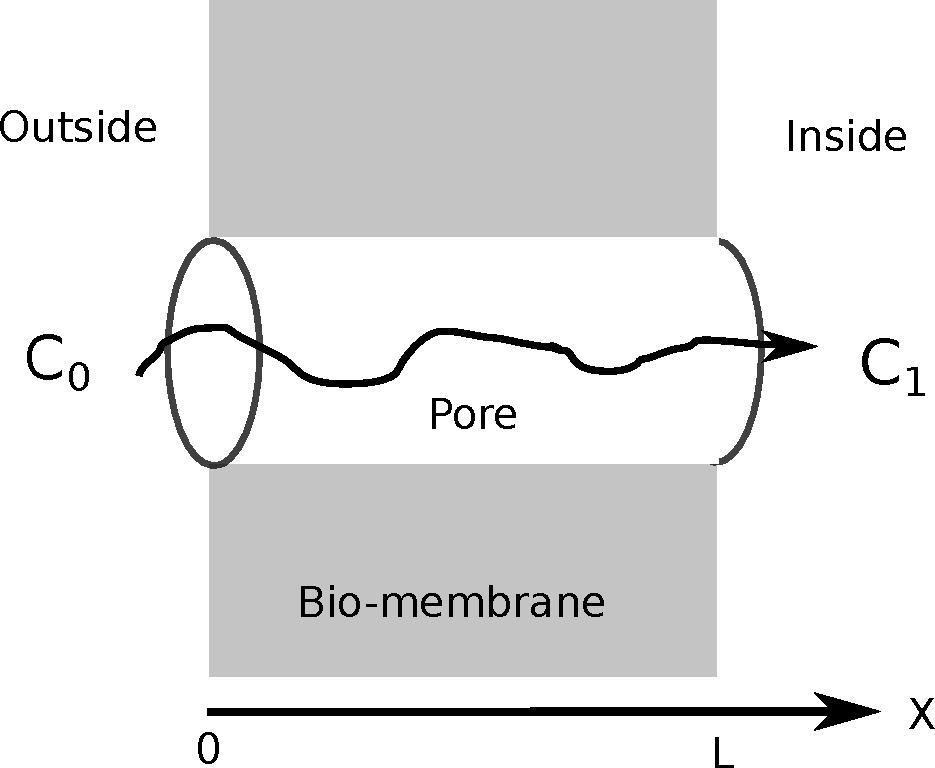
\includegraphics[scale=0.4]{figs/biopore.pdf}
      \caption{\label{fig:biopore}
        Illustration of the bio-pore.
      }
    \end{center}
  \end{figure}
  
  Let the steady-state concentration of C in the pore be denoted $c=c(x)$ where
  $0 \leq x \leq L$. The dynamics is modelled from the steady-state RD-equation
  with mixed BCs
  \begin{equation}
    \label{eq:rdss}
    r(c) + D \frac{\d^2c}{\d x^2} = 0 \ , \ c(0)=C_0 \ \ \text{and} \ \
    \left. \frac{\d c}{\d x}\right|_{x=L} =0 \, .
  \end{equation}
  
  \begin{enumerate}
  \item Show that the condition $C_0 > C_1$ cannot be met if the
    reaction term in Equation (\ref{eq:rdss}) is omitted. 
  \item Show that if $r(c)=-k_1c$ the concentration profile is given by
    \begin{equation}
      c(x) = C_0\left[
        e^{-\alpha L}\frac{\sinh(\alpha x)}{\cosh(\alpha L)} + e^{-\alpha x}
      \right] \, ,
    \end{equation}
    where $\alpha = \sqrt{k_1/D}$
  \item Now let $r(c)=-k_2c^2$. Find the solution up to first order in
    the perturbation parameter $\varepsilon = k_2/D$. Explain the
    fundamental physical unit that determines the validity of this
    approximate solution.
  \end{enumerate}
  \end{exploration}
\end{exerciseregion}

\section{Chemotaxis}
Experimentally it has been observed that some cells, e.g., E-coli, can
register (or sense) 
a chemical concentration gradient and move either down or up this gradient. 
The chemical compound can be a hormone and cell motion 
is realised by, for example, flagella propulsion. 
This phenomenon is denoted \emph{chemotaxis}. To model chemotaxis we need to
change the fluxes in the system. If diffusion and chemotaxis are independent processes we
can write the flux with two terms: (i) a term describing the usual diffusive flux 
and (ii) a term describing the flux due to chemotaxis. 

Consider a cell population with concentration $c_1=c_1(x,t)$ mixed with a
a chemical compound having concentration $c_2=c_2(x,t)$. The \emph{Keller-Segel
model} for the flux of the cells reads
\begin{eqnarray}
	J_1 = \chi c_1 \frac{\partial c_2}{\partial x} - D_1 \frac{\partial c_1}{\partial x} \, ,
\end{eqnarray}
where $\chi$ is the \emph{chemotactic strength} and $D_1$ the usual diffusion 
coefficient for the cells. What the two terms describe should be clear. If the chemotactic strength 
or the gradient of the chemical is zero, then, of course, no flux occurs due to chemotaxis. 
The product in the chemotaxis term between $c_1$ and $\partial c_2/\partial x$ give raise to a 
(potential) non-linearity, and ensures that there is no flux of cells at point when there are no
cells even if the gradient of the chemical is non-zero. Substitution into the 
balance equation for $c_1$ gives 	
\begin{eqnarray}
	\frac{\partial c_1}{\partial t} = r(c_1) - \chi \frac{\partial}{\partial x} \left( c_1 \frac{\partial c_2}{\partial x} \right)
	+ D_1 \frac{\partial^2c_1}{\partial x^2} 
\end{eqnarray}
if $\chi$ and $D_1$ are independent of spatial coordinate $x$. In the
steady-state this is simply
\begin{eqnarray}
	r(c_1) -\chi \frac{\d}{\d x} \left( c_1 \frac{\d c_2}{\d x}\right) + D_1
	\frac{\d ^2 c_1}{\d x^2} = 0 \, . 
\end{eqnarray}

\begin{question}
	Will the cells move up or down the chemical gradient if $\chi > 0$? What if $\chi <
	0$?
\end{question}

\begin{example}
	\label{ex:chemotaxis}
	Assume that we some how  can control the local concentration of the chemical compound.
	For example, let
	\begin{eqnarray}
		\label{eq:c2}
		c_2 = Kx/L  \ \text{such that} \ c_2(0)=0 \ \text{and} \ c_2(L) = K.
	\end{eqnarray}
	Let the cells feature a linear growth rate, $r = k c_1$, and use Dirichlet
	BCs $c_1(0) = C_0$ and $c_1(L) = 2C_0$, where $C_0 \neq 0$.  
	The equation (for the steady-state) is 	obtained using the product rule
	\begin{eqnarray}
		k c_1 -\chi \frac{\d}{\d x} \left( c_1 \frac{\d c_2}{\d x}\right) + D_1 \frac{\d ^2 c_1}{\d x^2} = 
		0 \ \Rightarrow \ 
		\frac{k}{D_1} c_1 - \frac{\chi K}{D_1 L} \frac{\d c_1}{\d x} +
		\frac{\d^2c_1}{\d x^2} =  0 \, . 
	\end{eqnarray}
	\begin{wrapfigure}[15]{R}{0.4\textwidth}
		\centering
		\includegraphics[width=0.35\textwidth]{figs/chemotaxis.eps}
		\caption*{}
	\end{wrapfigure}
	\paragraph{}
	\vspace*{-\parskip}
	Define the parameter $\alpha = \chi K/(D_1 L)$ then the characteristic polynomial is 
	\begin{eqnarray}
		\lambda^2 - \alpha \lambda + \frac{k}{D_1} = 0 \ ,
	\end{eqnarray}
	implying that 
	\begin{eqnarray}
		\lambda_{1,2} = \frac{1}{2}\left(
		\alpha \pm \sqrt{\alpha^2 - 4k/D_1}  \right) \, .
	\end{eqnarray}
	For real eigenvalues, $\alpha^2 > 4k/D_1$, we then have the general solution
	\begin{eqnarray}
		c_1(x) = A e^{\lambda_1 x} + B e^{\lambda_2 x} \, .
	\end{eqnarray}
	Applying the BCs we obtain
	\begin{eqnarray}
		c_1(x) = C_0 \left[
			e^{\lambda_1x} + \frac{2 - e^{\lambda_1 L}}{e^{\lambda_2L}-e^{\lambda_1 L}} 
			(e^{\lambda_2 x} - e^{\lambda_1 x})
		\right] \, . \nonumber \\
	\end{eqnarray}
	Note, by introducing chemotaxis the concentration profile can change from a
	concave function to a convex function depending on the sign of $\alpha$,
	that is, on the sign of the chemotactic strength, $\chi$.
\end{example}

In the general case, we may not be able to control the concentration of the
chemical compound and we then need a dynamical equation for $c_2$ as well.
Equation (\ref{eq:c2}) is equivalent to the case, where the chemical is not
consumed by the cells and simply diffuses according to Fick's law, that is,
$c_2$ follows the Laplace equation 
\begin{eqnarray}
	\frac{\d^2 c_2}{\d x^2} = 0 \ \text{with} \ c_2(0) = \ \text{and} \ c_2(L) =
	K \, .
\end{eqnarray}
We will not pursue the general case here.

\begin{exerciseregion}
	\begin{exercise}
		Solve the chemotaxis problem in Example \ref{ex:chemotaxis} for the
		situation where the reaction function is zero everywhere, $r=0$.
	\end{exercise}
	\begin{exercise}
		Consider a mixture of cells and a chemical compound. The system features
		chemotaxis, and we can measure the steady-state concentration of the cells to 
		\begin{eqnarray}
			c_1 = \frac{C_0}{L^2} x (x-L) \, ,
		\end{eqnarray}
		where $C_0$ is a reference concentration. Derive an expression for the
		steady concentration of the chemical assuming that no reactions occur.
	\end{exercise}
\end{exerciseregion}





















